% Options for packages loaded elsewhere
\PassOptionsToPackage{unicode}{hyperref}
\PassOptionsToPackage{hyphens}{url}
%
\documentclass[
  hyperref,]{ctexart}
\usepackage{amsmath,amssymb}
\usepackage{iftex}
\ifPDFTeX
  \usepackage[T1]{fontenc}
  \usepackage[utf8]{inputenc}
  \usepackage{textcomp} % provide euro and other symbols
\else % if luatex or xetex
  \usepackage{unicode-math} % this also loads fontspec
  \defaultfontfeatures{Scale=MatchLowercase}
  \defaultfontfeatures[\rmfamily]{Ligatures=TeX,Scale=1}
\fi
\usepackage{lmodern}
\ifPDFTeX\else
  % xetex/luatex font selection
\fi
% Use upquote if available, for straight quotes in verbatim environments
\IfFileExists{upquote.sty}{\usepackage{upquote}}{}
\IfFileExists{microtype.sty}{% use microtype if available
  \usepackage[]{microtype}
  \UseMicrotypeSet[protrusion]{basicmath} % disable protrusion for tt fonts
}{}
\makeatletter
\@ifundefined{KOMAClassName}{% if non-KOMA class
  \IfFileExists{parskip.sty}{%
    \usepackage{parskip}
  }{% else
    \setlength{\parindent}{0pt}
    \setlength{\parskip}{6pt plus 2pt minus 1pt}}
}{% if KOMA class
  \KOMAoptions{parskip=half}}
\makeatother
\usepackage{xcolor}
\usepackage[left=2.5cm,right=2cm,top=3cm,bottom=2.5cm]{geometry}
\usepackage{color}
\usepackage{fancyvrb}
\newcommand{\VerbBar}{|}
\newcommand{\VERB}{\Verb[commandchars=\\\{\}]}
\DefineVerbatimEnvironment{Highlighting}{Verbatim}{commandchars=\\\{\}}
% Add ',fontsize=\small' for more characters per line
\usepackage{framed}
\definecolor{shadecolor}{RGB}{248,248,248}
\newenvironment{Shaded}{\begin{snugshade}}{\end{snugshade}}
\newcommand{\AlertTok}[1]{\textcolor[rgb]{0.94,0.16,0.16}{#1}}
\newcommand{\AnnotationTok}[1]{\textcolor[rgb]{0.56,0.35,0.01}{\textbf{\textit{#1}}}}
\newcommand{\AttributeTok}[1]{\textcolor[rgb]{0.13,0.29,0.53}{#1}}
\newcommand{\BaseNTok}[1]{\textcolor[rgb]{0.00,0.00,0.81}{#1}}
\newcommand{\BuiltInTok}[1]{#1}
\newcommand{\CharTok}[1]{\textcolor[rgb]{0.31,0.60,0.02}{#1}}
\newcommand{\CommentTok}[1]{\textcolor[rgb]{0.56,0.35,0.01}{\textit{#1}}}
\newcommand{\CommentVarTok}[1]{\textcolor[rgb]{0.56,0.35,0.01}{\textbf{\textit{#1}}}}
\newcommand{\ConstantTok}[1]{\textcolor[rgb]{0.56,0.35,0.01}{#1}}
\newcommand{\ControlFlowTok}[1]{\textcolor[rgb]{0.13,0.29,0.53}{\textbf{#1}}}
\newcommand{\DataTypeTok}[1]{\textcolor[rgb]{0.13,0.29,0.53}{#1}}
\newcommand{\DecValTok}[1]{\textcolor[rgb]{0.00,0.00,0.81}{#1}}
\newcommand{\DocumentationTok}[1]{\textcolor[rgb]{0.56,0.35,0.01}{\textbf{\textit{#1}}}}
\newcommand{\ErrorTok}[1]{\textcolor[rgb]{0.64,0.00,0.00}{\textbf{#1}}}
\newcommand{\ExtensionTok}[1]{#1}
\newcommand{\FloatTok}[1]{\textcolor[rgb]{0.00,0.00,0.81}{#1}}
\newcommand{\FunctionTok}[1]{\textcolor[rgb]{0.13,0.29,0.53}{\textbf{#1}}}
\newcommand{\ImportTok}[1]{#1}
\newcommand{\InformationTok}[1]{\textcolor[rgb]{0.56,0.35,0.01}{\textbf{\textit{#1}}}}
\newcommand{\KeywordTok}[1]{\textcolor[rgb]{0.13,0.29,0.53}{\textbf{#1}}}
\newcommand{\NormalTok}[1]{#1}
\newcommand{\OperatorTok}[1]{\textcolor[rgb]{0.81,0.36,0.00}{\textbf{#1}}}
\newcommand{\OtherTok}[1]{\textcolor[rgb]{0.56,0.35,0.01}{#1}}
\newcommand{\PreprocessorTok}[1]{\textcolor[rgb]{0.56,0.35,0.01}{\textit{#1}}}
\newcommand{\RegionMarkerTok}[1]{#1}
\newcommand{\SpecialCharTok}[1]{\textcolor[rgb]{0.81,0.36,0.00}{\textbf{#1}}}
\newcommand{\SpecialStringTok}[1]{\textcolor[rgb]{0.31,0.60,0.02}{#1}}
\newcommand{\StringTok}[1]{\textcolor[rgb]{0.31,0.60,0.02}{#1}}
\newcommand{\VariableTok}[1]{\textcolor[rgb]{0.00,0.00,0.00}{#1}}
\newcommand{\VerbatimStringTok}[1]{\textcolor[rgb]{0.31,0.60,0.02}{#1}}
\newcommand{\WarningTok}[1]{\textcolor[rgb]{0.56,0.35,0.01}{\textbf{\textit{#1}}}}
\usepackage{graphicx}
\makeatletter
\def\maxwidth{\ifdim\Gin@nat@width>\linewidth\linewidth\else\Gin@nat@width\fi}
\def\maxheight{\ifdim\Gin@nat@height>\textheight\textheight\else\Gin@nat@height\fi}
\makeatother
% Scale images if necessary, so that they will not overflow the page
% margins by default, and it is still possible to overwrite the defaults
% using explicit options in \includegraphics[width, height, ...]{}
\setkeys{Gin}{width=\maxwidth,height=\maxheight,keepaspectratio}
% Set default figure placement to htbp
\makeatletter
\def\fps@figure{htbp}
\makeatother
\setlength{\emergencystretch}{3em} % prevent overfull lines
\providecommand{\tightlist}{%
  \setlength{\itemsep}{0pt}\setlength{\parskip}{0pt}}
\setcounter{secnumdepth}{-\maxdimen} % remove section numbering
\ifLuaTeX
  \usepackage{selnolig}  % disable illegal ligatures
\fi
\IfFileExists{bookmark.sty}{\usepackage{bookmark}}{\usepackage{hyperref}}
\IfFileExists{xurl.sty}{\usepackage{xurl}}{} % add URL line breaks if available
\urlstyle{same}
\hypersetup{
  pdftitle={2151299\_苏家铭\_hw2},
  pdfauthor={苏家铭},
  hidelinks,
  pdfcreator={LaTeX via pandoc}}

\title{2151299\_苏家铭\_hw2}
\author{苏家铭}
\date{}

\begin{document}
\maketitle

This is an \href{http://rmarkdown.rstudio.com}{R Markdown} Notebook.
When you execute code within the notebook, the results appear beneath
the code.

Try executing this chunk by clicking the \emph{Run} button within the
chunk or by placing your cursor inside it and pressing
\emph{Ctrl+Shift+Enter}.

\begin{Shaded}
\begin{Highlighting}[]
\CommentTok{\# Body piercing data}
\NormalTok{american.bp }\OtherTok{\textless{}{-}} \FunctionTok{c}\NormalTok{(}\DecValTok{3}\NormalTok{, }\DecValTok{5}\NormalTok{, }\DecValTok{2}\NormalTok{, }\DecValTok{1}\NormalTok{, }\DecValTok{4}\NormalTok{, }\DecValTok{4}\NormalTok{, }\DecValTok{6}\NormalTok{, }\DecValTok{3}\NormalTok{, }\DecValTok{5}\NormalTok{, }\DecValTok{4}\NormalTok{)}
\NormalTok{european.bp }\OtherTok{\textless{}{-}} \FunctionTok{c}\NormalTok{(}\DecValTok{6}\NormalTok{, }\DecValTok{5}\NormalTok{, }\DecValTok{7}\NormalTok{, }\DecValTok{7}\NormalTok{, }\DecValTok{6}\NormalTok{, }\DecValTok{3}\NormalTok{, }\DecValTok{4}\NormalTok{, }\DecValTok{6}\NormalTok{, }\DecValTok{5}\NormalTok{, }\DecValTok{4}\NormalTok{)}
\CommentTok{\# Store data in a datafram}
\NormalTok{ebp.survey }\OtherTok{\textless{}{-}} \FunctionTok{data.frame}\NormalTok{(}\StringTok{"bp"} \OtherTok{=} \FunctionTok{c}\NormalTok{(american.bp, european.bp),}
\StringTok{"group"} \OtherTok{=} \FunctionTok{rep}\NormalTok{(}\FunctionTok{c}\NormalTok{(}\StringTok{"American"}\NormalTok{,}\StringTok{"European"}\NormalTok{), }\AttributeTok{each =} \DecValTok{10}\NormalTok{),}\AttributeTok{stringsAsFactors =} \ConstantTok{FALSE}\NormalTok{)}
\end{Highlighting}
\end{Shaded}

\begin{Shaded}
\begin{Highlighting}[]
\CommentTok{\# 导入pirates包}
\FunctionTok{load}\NormalTok{(}\StringTok{"pirates.RData"}\NormalTok{)}
\end{Highlighting}
\end{Shaded}

\begin{Shaded}
\begin{Highlighting}[]
\FunctionTok{library}\NormalTok{(yarrr)}
\end{Highlighting}
\end{Shaded}

\begin{verbatim}
## 载入需要的程辑包:jpeg
\end{verbatim}

\begin{verbatim}
## 载入需要的程辑包:BayesFactor
\end{verbatim}

\begin{verbatim}
## 载入需要的程辑包:coda
\end{verbatim}

\begin{verbatim}
## 载入需要的程辑包:Matrix
\end{verbatim}

\begin{verbatim}
## ************
## Welcome to BayesFactor 0.9.12-4.5. If you have questions, please contact Richard Morey (richarddmorey@gmail.com).
## 
## Type BFManual() to open the manual.
## ************
\end{verbatim}

\begin{verbatim}
## 载入需要的程辑包:circlize
\end{verbatim}

\begin{verbatim}
## ========================================
## circlize version 0.4.15
## CRAN page: https://cran.r-project.org/package=circlize
## Github page: https://github.com/jokergoo/circlize
## Documentation: https://jokergoo.github.io/circlize_book/book/
## 
## If you use it in published research, please cite:
## Gu, Z. circlize implements and enhances circular visualization
##   in R. Bioinformatics 2014.
## 
## This message can be suppressed by:
##   suppressPackageStartupMessages(library(circlize))
## ========================================
\end{verbatim}

\begin{verbatim}
## yarrr v0.1.5. Citation info at citation('yarrr'). Package guide at yarrr.guide()
\end{verbatim}

\begin{verbatim}
## Email me at Nathaniel.D.Phillips.is@gmail.com
\end{verbatim}

\begin{Shaded}
\begin{Highlighting}[]
\FunctionTok{pirateplot}\NormalTok{(bp }\SpecialCharTok{\textasciitilde{}}\NormalTok{ group, }\AttributeTok{data =}\NormalTok{ ebp.survey, }\AttributeTok{main =} \StringTok{"海盗身体穿孔数目"}\NormalTok{, }\AttributeTok{xlab =} \StringTok{"地区"}\NormalTok{, }\AttributeTok{ylab =} \StringTok{"穿孔数目"}\NormalTok{)}
\end{Highlighting}
\end{Shaded}

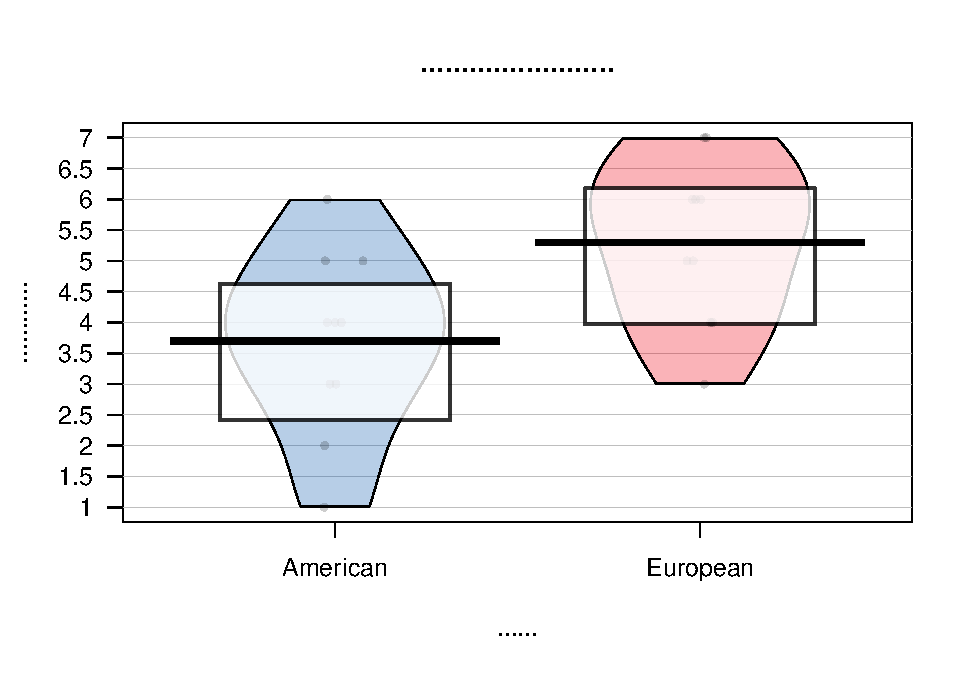
\includegraphics{2151299_苏家铭_hw2_files/figure-latex/step1-1.pdf}

\begin{Shaded}
\begin{Highlighting}[]
\CommentTok{\# 中位数(Median): 箱线图的矩形框中线表示数据的中位数。观察中位数可以得知数据的中心趋势。欧洲的中位数比美国的高表示欧洲海盗穿孔中间值比美国的大。}

\CommentTok{\# 四分位数(Quartiles): 箱线图显示了数据的上下四分位数,即数据的前25\%和后25\%的范围。箱体的上下边缘表示第三四分位数(Q3)和第一四分位数(Q1),而箱子的高度表示数据的中间50\%范围。欧洲的四分位数也比美国高。}

\CommentTok{\# 箱子的长度: 箱子的长度(IQR,即四分位距)表示数据的离散程度,即在四分位数范围内的数据分布情况。离散程度相差无几。}

\CommentTok{\# 综合来看,欧洲海盗比美国海盗身体穿孔数目更多。}
\end{Highlighting}
\end{Shaded}

\begin{Shaded}
\begin{Highlighting}[]
\CommentTok{\# 步骤 2: t{-}test}
\NormalTok{p.test\_result }\OtherTok{\textless{}{-}} \FunctionTok{t.test}\NormalTok{(bp }\SpecialCharTok{\textasciitilde{}}\NormalTok{ group, }\AttributeTok{data =}\NormalTok{ ebp.survey)}
\FunctionTok{print}\NormalTok{(p.test\_result)}
\end{Highlighting}
\end{Shaded}

\begin{verbatim}
## 
##  Welch Two Sample t-test
## 
## data:  bp by group
## t = -2.5228, df = 17.783, p-value = 0.0214
## alternative hypothesis: true difference in means between group American and group European is not equal to 0
## 95 percent confidence interval:
##  -2.9335927 -0.2664073
## sample estimates:
## mean in group American mean in group European 
##                    3.7                    5.3
\end{verbatim}

\begin{Shaded}
\begin{Highlighting}[]
\CommentTok{\# t{-}statistic ({-}2.5228): t{-}statistic为负值,表示"American"组的样本均值较小。}

\CommentTok{\# 自由度 (df = 17.783): 这是一个衡量我们有多少信息来估计总体方差的指标。由于Welch\textquotesingle{}s t{-}test考虑到了两组方差不一致的情况,因此自由度被修正为一个小数。}

\CommentTok{\# p{-}value (0.0214): 在这里,p{-}value小于通常选择的显著性水平(通常是0.05),因此我们拒绝了零假设。这意味着我们有足够的证据表明"American"组和"European"组的平均穿孔数目是显著不同的。}

\CommentTok{\# 95 percent confidence interval ({-}2.9335927,{-}0.2664073):在这里,置信区间不包括零,这进一步支持我们对显著性差异的结论。负的区间下限表明"American"组的平均值可能小于"European"组。}

\CommentTok{\# 综合来说,根据这个t{-}test的结果,我们有理由相信"American"组和"European"组的平均穿孔数目是不同的。}
\end{Highlighting}
\end{Shaded}

\begin{Shaded}
\begin{Highlighting}[]
\CommentTok{\# 提取 29 岁和 30 岁的海盗的文身数量}
\NormalTok{tattoos\_29 }\OtherTok{\textless{}{-}}\NormalTok{ pirates}\SpecialCharTok{$}\NormalTok{tattoos[pirates}\SpecialCharTok{$}\NormalTok{age }\SpecialCharTok{==} \DecValTok{29}\NormalTok{]}
\NormalTok{tattoos\_30 }\OtherTok{\textless{}{-}}\NormalTok{ pirates}\SpecialCharTok{$}\NormalTok{tattoos[pirates}\SpecialCharTok{$}\NormalTok{age }\SpecialCharTok{==} \DecValTok{30}\NormalTok{]}

\CommentTok{\# 进行 t 检验}
\NormalTok{t.test\_result }\OtherTok{\textless{}{-}} \FunctionTok{t.test}\NormalTok{(tattoos\_29, tattoos\_30)}

\CommentTok{\# 查看 t{-}test 结果}
\FunctionTok{print}\NormalTok{(t.test\_result)}
\end{Highlighting}
\end{Shaded}

\begin{verbatim}
## 
##  Welch Two Sample t-test
## 
## data:  tattoos_29 and tattoos_30
## t = 0.26552, df = 119.15, p-value = 0.7911
## alternative hypothesis: true difference in means is not equal to 0
## 95 percent confidence interval:
##  -1.058586  1.386455
## sample estimates:
## mean of x mean of y 
## 10.081967  9.918033
\end{verbatim}

\begin{Shaded}
\begin{Highlighting}[]
\CommentTok{\# t{-}statistic (0.26552): t{-}statistic接近零,说明观察到的均值差异相对较小。}

\CommentTok{\#自由度 (df = 119.15): 由于Welch\textquotesingle{}st{-}test考虑到了两组方差不一致的情况,因此自由度被修正为一个小数。}

\CommentTok{\# p{-}value (0.7911): 这是一个衡量观察到的样本均值差异是否由于随机变异引起的指标。在这里,p{-}value很大,大于通常选择的显著性水平(通常是0.05),因此我们没有足够的证据拒绝零假设。这意味着我们没有足够的证据表明 29 岁和 30 岁海盗的文身数量存在显著差异。}

\CommentTok{\# 95 percent confidence interval ({-}1.058586, 1.386455): 这是对真实均值差异的估计区间。由于包含零,这意味着我们对真实差异的估计不显著。}

\CommentTok{\# 综合来看,根据这个t{-}test的结果,我们没有足够的证据来支持 29 岁和 30 岁海盗的文身数量存在显著差异的假设。p{-}value 大,置信区间包含零,都支持这一结论。}
\end{Highlighting}
\end{Shaded}

\begin{Shaded}
\begin{Highlighting}[]
\CommentTok{\# 创建一个列联表}
\NormalTok{cross\_table }\OtherTok{\textless{}{-}} \FunctionTok{table}\NormalTok{(pirates}\SpecialCharTok{$}\NormalTok{eyepatch, pirates}\SpecialCharTok{$}\NormalTok{college)}

\CommentTok{\# 进行卡方检验}
\NormalTok{c.test }\OtherTok{\textless{}{-}} \FunctionTok{chisq.test}\NormalTok{(cross\_table)}

\CommentTok{\# 查看卡方检验结果}
\FunctionTok{print}\NormalTok{(c.test)}
\end{Highlighting}
\end{Shaded}

\begin{verbatim}
## 
##  Pearson's Chi-squared test with Yates' continuity correction
## 
## data:  cross_table
## X-squared = 0, df = 1, p-value = 1
\end{verbatim}

\begin{Shaded}
\begin{Highlighting}[]
\CommentTok{\# X{-}squared (0): X{-}squared 为 0,表明观察到的频数与期望频数非常接近,没有显著的偏离。}

\CommentTok{\# 自由度 (df = 1): 这是卡方分布的自由度。对于 Pearson\textquotesingle{}s Chi{-}squared test,自由度是 (行数 {-} 1) * (列数 {-} 1)。在这里,由于只有两个列(\textquotesingle{}CCCC\textquotesingle{} 和 \textquotesingle{}JSSFP\textquotesingle{}),因此自由度为 1。}

\CommentTok{\# p{-}value (1): 这是检验的 p{-}value,用于判断观察到的频数与期望频数之间的差异是否显著。在这里,p{-}value 等于1,这说明我们没有足够的证据拒绝零假设,即是否佩戴眼罩与所上大学之间没有显著关联。}

\CommentTok{\# 总体上,根据这个卡方检验的结果,我们没有足够的证据支持是否佩戴眼罩与所上大学之间存在显著关联的假设。}
\end{Highlighting}
\end{Shaded}

Add a new chunk by clicking the \emph{Insert Chunk} button on the
toolbar or by pressing \emph{Ctrl+Alt+I}.

When you save the notebook, an HTML file containing the code and output
will be saved alongside it (click the \emph{Preview} button or press
\emph{Ctrl+Shift+K} to preview the HTML file).

The preview shows you a rendered HTML copy of the contents of the
editor. Consequently, unlike \emph{Knit}, \emph{Preview} does not run
any R code chunks. Instead, the output of the chunk when it was last run
in the editor is displayed.

\end{document}
